% !TEX TS-program = pdflatex
% !TEX encoding = UTF-8 Unicode

% This is a simple template for a LaTeX document using the "article" class.
% See "book", "report", "letter" for other types of document.

\documentclass[11pt]{article} % use larger type; default would be 10pt
\usepackage[a4paper, top=20mm, left =20mm, right =20mm ,bottom=20mm ]{geometry}
\usepackage{lineno}
\modulolinenumbers[1]
\journal{TRE}
\usepackage{graphicx}
\usepackage{ulem}
\usepackage{array}
\usepackage{epstopdf}
\usepackage{amstext}
\usepackage[utf8]{inputenc}
\usepackage[english]{babel}
\usepackage{amsfonts}
\usepackage{color}
\usepackage{amssymb}
\usepackage[citecolor=blue,linkcolor=blue,colorlinks=true]{hyperref}
\usepackage{multirow}
\usepackage{amsmath}
%\usepackage{lmodern}
%\usepackage{booktabs}
\usepackage{float}
\usepackage{tabularx}
\usepackage{geometry}
\usepackage{lscape}
\usepackage{longtable}
\usepackage{romannum}
\usepackage{makecell}
\usepackage{adjustbox}
\usepackage{lscape} 
%\usepackage{hyperref}

\usepackage{booktabs}

\usepackage{cleveref}
\usepackage{tablefootnote}
\crefformat{footnote}{#2\footnotemark[#1]#3}
\usepackage{blindtext}
\usepackage{algorithmicx,algpseudocode}
\usepackage[linesnumbered,ruled]{algorithm2e}
\usepackage{amsthm} % add by zhou
\newtheorem{theorem}{Theorem} % add by zhou
 
%\usepackage{longtable}
%\usepackage{natbib} 
%\usepackage[super,square]{natbib} 
\usepackage{longtable} 
\usepackage{float}
\usepackage{footnote}
\renewcommand{\thefootnote}{\arabic{footnote}}
%\pagenumbering{Roman} 
\pagenumbering{arabic} 
\newtheorem{definition}{Definition}
%\newcommand{\red}[1]{\textcolor{red}{#1}}
%%%%%%%%%%%%%%%%%%%%%%%
%% Elsevier bibliography styles
%%%%%%%%%%%%%%%%%%%%%%%
%% To change the style, put a % in front of the second line of the current style and
%% remove the % from the second line of the style you would like to use.
%%%%%%%%%%%%%%%%%%%%%%%
%% Numbered
%\bibliographystyle{model1-num-names}

%% Numbered without titles
%\bibliographystyle{model1a-num-names}

%% Harvard
% \bibliographystyle{model2-names.bst}\biboptions{authoryear}
%% Vancouver numbered
%\usepackage{numcompress}\bibliographystyle{model3-num-names}

%% Vancouver name/year
%\usepackage{numcompress}\bibliographystyle{model4-names}\biboptions{authoryear}

%% APA style
%\bibliographystyle{model5-names}
%\biboptions{authoryear}
%\bibliographystyle{apa}
%% AMA style
%\usepackage{numcompress}\bibliographystyle{model6-num-names}

%% `Elsevier LaTeX' style
%\bibliographystyle{elsarticle-num}
%%%%%%%%%%%%%%%%%%%%%%%
%\bibliographystyle{apalike}
\newlength\mylength
\renewcommand{\baselinestretch}{1.5}
% 
% 
% 
% 
% 
% 
% 
% 
% 
% 
% 
% 
% 

% 
\title{Insights for Auto Port Ranking with LangChain-LLMs}
\author{\textbf{Zehao Qian} \ \ \ \href{mailto:zehao.qian.cn@gmail.com}{zehao.qian.cn@gmail.com}}
\begin{document}
\maketitle
% 
% 
% 
% \tableofcontents
% 
% 
% 
% 
\section{Task Schedule Model}
% 
\begin{figure}[H]
    \centering
    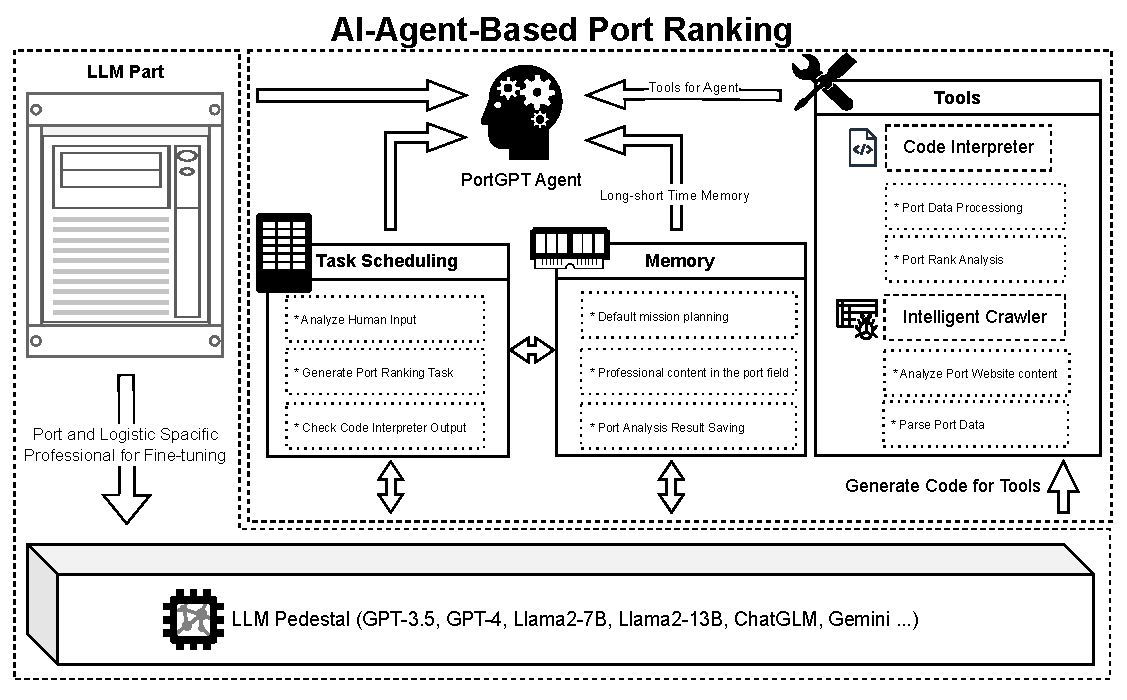
\includegraphics[width=1.0\textwidth]{pic/PortGPT.pdf}
    \caption{PortGPT Conceptual Architecture}
    \label{fig:PortGPT}
\end{figure}
%
% 
% 
% 
% 
% 
\section{LLM Fine-tuning and Prompt Engineering for Auto Port Ranking}
% 
% 
% 
% 
% 
\section{Port Data Acquisition}
% 
% 
\begin{longtable}{
    >{\raggedright\arraybackslash}m{0.3\textwidth}
    >{\raggedright\arraybackslash}m{0.35\textwidth}
    >{\raggedright\arraybackslash}m{0.35\textwidth}
}
    \hline
    \textbf{Type}                     & \textbf{Advantages} & \textbf{Disadvantages} \\
    \hline
    \endfirsthead

    \hline
    \textbf{Type}                     & \textbf{Advantages} & \textbf{Disadvantages} \\
    \hline
    \endhead

    \hline
    \endfoot

    \hline
    Traditional Web Crawlers          &
    - Fast speed\newline
    - Low resource consumption\newline
    - Simple and easy to use          &
    - Poor flexibility\newline
    - Easily blocked by anti-crawling mechanisms                                     \\
    \hline
    Selenium-based Crawlers           &
    - Highly flexible\newline
    - Can handle complex scenarios    &
    - Slower speed\newline
    - High resource consumption\newline
    - High complexity                                                                \\
    \hline
    LLM-based Intelligent Crawlers    &
    - Strong understanding ability\newline
    - Strong adaptability\newline
    - Capable of complex interactions &
    - Potential speed limitations\newline
    - Resource-intensive\newline
    - Challenges in accuracy                                                         \\
    \hline
\end{longtable}
% 
% 
% 
% 
\section{Dealing with Outliers and Missing Values}
% 
% 
% 
% 
% 
% 
% 
% 
% 
\subsection{Outliers}
% 
% 
% 
% 
% 
% 
% 
% 
% 
% 
% 
\subsection{Missing Values}
% 
% 
% 
% 这部分讨论了现代港口管理和运筹学中数据完整性和准确性的重要性,特别关注了数据缺失的问题及其影响。研究首先分析了港口数据缺失的模式和原因,然后探讨了处理数据缺失的不同策略,主要包括插补法和删除法。这部分强调,在选择删除或插补数据时,需要考虑数据缺失的比例和模式、数据性质、分析方法的要求以及研究目的,以确保分析结果的准确性和可靠性。
% 
% 
% 
\paragraph{In modern port management and Operation Research, the integrity and accuracy of data is very important. Effective data analysis can not only reveal the current state of port operation, but also predict future trends and potential problems. However, data loss is a common problem in data collection, which can be caused by a number of factors, including technical failures, recording errors or delayed information updates. The purpose of this paper is to explore and solve this challenge in order to enhance the understanding and application of port data.}
% 
% 
% 
% 
% 
% 
\paragraph{Firstly, the data collected from the port were examined to identify the patterns and possible causes of missing data. On this basis, we will explore various strategies to deal with missing data to ensure the accuracy and reliability of the analysis results. We will focus in particular on two major approaches: Imputation and Deletion. The interpolation method aims at estimating missing values and filling data gaps with these estimates, while the deletion method is to remove data records containing missing values.}
% 
% 
% 
\paragraph{\textbf{Delete or Impute?} When deciding whether to delete or impute missing data, consider the proportion and pattern of missingness, the nature of the data, the requirements of the analysis method, and the purpose of the study. Deletion is suitable for small proportions of randomly missing data and when it won't introduce bias, while imputation is preferred for large proportions of missing data, non-random missingness, to maintain dataset size and integrity, and to retain critical information. The decision should balance the characteristics of the data, the reasons for missingness, and the objectives of the analysis. \cite{Jakobsen2017}}
% 
% 
% 
% 
\subsubsection{Tranditional Missing Data Imputation Methods}
% 
% 
% 
\paragraph{\textbf{Mean/Median/Mode Imputation} \cite{Kleinbort2020} is a common and simple method where all missing values are replaced with the mean, median, or mode of the column. Although this approach is easy and fast, it has its drawbacks. It can skew the statistical nature of the data, underestimate variance, and distort histograms. This method is generally advisable only when data is missing completely at random (MCAR) or missing at random (MAR), but it is not suitable if data is missing not at random (MNAR)}
% 
% 
% 
\paragraph{\textbf{Multiple Imputation} \cite{Sterneb2393} \cite{Khan2020} involves creating multiple copies of the dataset, where missing values are replaced with imputed values based on their predictive distribution from observed data. This method uses standard statistical methods to fit models to each imputed dataset, and then averages the results to provide overall estimated associations. Multiple imputation, based on a Bayesian approach, accounts for all uncertainty in predicting missing values by introducing appropriate variability into the imputed values. It is essential in multiple imputation to model the distribution of each variable with missing values accurately. However, pitfalls can occur, such as omitting the outcome variable from the imputation process or dealing incorrectly with non-normally distributed variables. The validity of results from multiple imputation depends on careful and appropriate modeling.}
% 
% 
% 
% 
% 
\paragraph{\textbf{KNN and linear regression imputing} \cite{10.1371/journal.pone.0295632} \cite{articleLearnKNN} \cite{inproceedingsKNearest} \cite{Emmanuel2021}}
% 
% 
% 
% 
% 
\subsubsection{Imputing Missing Data with Deep Learning and LLMs}
% 
% 
% 
% 
\paragraph{The great potential of deep learning in imputation of missing values in data. In the field of port management, these methods can be used to process and analyze large amounts of complex data, such as cargo flows, vessel dynamics, weather conditions, and port operation efficiency. Data imputation using deep learning not only improves data completeness and accuracy, but also helps predict and optimize port operations, thereby improving efficiency and safety. \cite{9458712} \cite{wang2022deep} \cite{park2022longterm} \cite{camino2019improving}}
% 
% 
% 
% 
% 
% 
\paragraph{In order to overcome the challenge of missing values in port data, this study proposes a method to predict and interpolate these missing values using a pre-trained model Xi machine learning. We first use existing port data, including multi-dimensional information such as cargo throughput, vessel arrival frequency, weather conditions, and port facility usage, to train our machine Xi model. This data has been cleaned and preprocessed to ensure the quality of the data fed into the model.
We chose a machine Xi model suitable for working with time series data, such as long short-term memory networks (LSTMs) or gated recurrent units (GRUs), because port data often have significant time-dependent and seasonal characteristics. The training of the model was performed on a rich historical dataset containing complete and missing instances of data collected from normal operations. In this way, the model learns Xi complex patterns and associations in the data, which can be used to predict missing values.}
% 
% 
% 
% 
% 
% 
% 
% 
% 
% 
% 
% 
% 
% 
% 
% 
% 
% 
% 
% 
% 
% 
% 
% 
% 
% 
% 
% 
% 
% 
% 
% 
% 
% 
% 
% 
% 
% 
\bibliographystyle{unsrt}
\bibliography{References}
% 
% 
% 
% 
% 
% 
% 
% 
\end{document}
